\section{Shor's Algorithm}
Shor's Algorithm allows us to solve integer factorization problem in polynomial time using quantum computer. That is, given integer N the algorithm finds the set of all prime factors of N - prime number that divide N. Many attempts have been made to find a classical, polynomial algorithm with no apparent success, the best known classical solution is roughly $O(2^{(\log N)^{1/3}})$ \cite{thebook}, as a result Shor's algorithm is considered the strongest premise that $\mathtt{BQP}$ is not equal to $\mathtt{BPP}$.
\subsection{Reduction to order-finding}
To achieve such an astounding reduction in complexity we have to reduce our problem of finding prime factors to a simpler problem. We easily see that to find all prime factors it is sufficient to be able to find a single non trivial prime factor, divide the original number by it and run the algorithm again. If we continue this procedure and store found factors we will solve the original problem as every number has a unique prime factorization.
\\\\
We now want to reduce this problem further to the problem of order finding. For a number $N$ we take a random value $a$ from the set of $\{2,\dots,N-1\}$. If we find the smallest number $s$ such that
\begin{align*}
    a^s=1\mod{N}
\end{align*}
that is, find the period of $a$ and assume that $s$ is odd than we can rewrite it as
\begin{align*}
    a^s-1&=0 \mod{N}\\
    (a^{s/2}+1)(a^{s/2}-1)&=0 \mod{N}\\
    (a^{s/2}+1)(a^{s/2}-1)&=kN
\end{align*}
now, if $a^{s/2}<N$ then we now that
\begin{align*}
    N|(a^{s/2}-1)(a^{s/2}+1)
\end{align*}
Note that from the condition $a^{s/2}<N$ one could assume that $a^{s/2}+1$ can be $N$, however this would imply that $a^{s/2}=1 \mod{N}$, which contradicts the fact that $s$ is the smallest number for which $a^{s}=1 \mod{N}$. Therefore both $\gcd(a^{s/2}\pm 1,N)<N$.
\\\\
From this we see that $\gcd(a^{s/2}\pm 1,N)$ are a factors of $N$, which we can compute classically, in polynomial time using Euclid's algorithm.\\\\
During the process we made two assumptions, $s$ is even and $a^{s/2}\neq \pm 1 \mod{N}$. Both of those conditions are easily checked classically, we can also bound the probability of it not happening (s being valid) to be at least 1/4 \cite{thebook}. If it happens, we simply choose different $a$ and repeat the process. 
\\\\
We see that we reduced our factoring problem to the order finding problem - finding the order of a number in $\mathbb{Z}_N$. This problem itself is also $\mathtt{NP}$-hard using classical approach, however we can exploit quantum Fourier transform to prove that it belongs to $\mathtt{BQP}$.
\subsection{Quantum Fourier Transform}
To lower down the complexity of order-finding we will utilize a variant of Fourier Transform over the group $\mathbb{Z}_N$, where $N=0^n$, which is a unitary operation over $\complex^{2^n}$. We present a way to implement it using $O(n^2)$ quantum gates which is exponentially faster than a classical approach, using FFT would take $O(n2^n)$ \cite{cormen2009}. However classical FFT outputs a vector from which we can read the result in its entirety, whereas QFT outputs an entangled quantum register that represents the same result, but upon measurement some information is lost. We cannot retrieve the full result, which means that QFT is only viable for certain applications. Luckily, one of them is order-finding.
\\\\
The Quantum Fourier Transform is formally defined by the operation acting on a qubit belonging to the quantum register of length $n$, as
\begin{align*}
    QFT(\ket{x})=\frac{1}{\sqrt{N}}\sum_{y=1}^{N} e^{2\pi i xy/N}\ket{y}
\end{align*}
We will compute it sequentially for each qubit, for $i$-th qubit we first apply a Hadamard gate on it to allow quantum interference, next we apply $n-i$ controlled phase gates to qubit $i$ taking qubits $\{i+1, n\}$ as control. Controlled phase gates take two qubits, target and control and apply a phase shift $e^{\pi / 2^k}$ to the target qubit if the control qubit is in state $\ket{1}$, where $k$ denotes the distance between qubits, we attach a visualization of the quantum circuit for $3$ qubit system \ref{fig:qft}.
\begin{figure}[ht!]
    \centering
    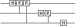
\includegraphics[width=0.7\linewidth]{figures/qft.pdf}
    \caption{QFT diagram for an example, 3 qubit system}
    \label{fig:qft}
\end{figure}

\subsection{Order finding}
We present a quantum algorithm that, given $a$ and $n$ such that $a<n, \gcd(a,n)=1$ on input, finds $r$ such that $a ^r=1 \mod n$. In other words, it finds the order of $a$ in group $\mathbb{Z}_n^*$, it's corresponding quantum circuit is presented on figure \ref{fig:shor}.
\\\\
In the algorithm we use two quantum registers. first will hold the value $a^x \mod n$ and the second will store the exponent $x$, initially both registers are set to ground state. As we need to utilize QFT, the registers' lengths need to be powers of 2; $m=\lceil\log n\rceil$.\\\\
first we initialize the first register with $m$ Hadamard gates, so it is in superposition of all possible $x$ resulting in a state:
\begin{align*}
    \ket{\xi}=\frac{1}{\sqrt{m}}\sum_{x=0}^{m-1}\ket{x}\ket{1}
\end{align*}
then we compute the function $f(x)=a^x \: \text{mod}\: n$, and put the result in the second register resulting in:
\begin{align*}
    \ket{\xi}=\frac{1}{\sqrt{m}}\sum_{x=0}^{m-1}\ket{x}\ket{a^x\: \text{mod}\: n}
\end{align*}
then we measure the second register to get value $y_0$. as we know the value in the second register, value in the first register is restricted so that $a^x \mod{n}=y_0$. it can be thus written as $x_0+lr$, where $x_0$ is the smallest x sufficing the condition, the current state is then:
\begin{align*}
  \ket{\xi}=\frac{1}{\sqrt{\lceil m/r \rceil}}\sum_{l=0}^{\lceil m/r \rceil-1}\ket{x_0 + lr}\ket{y_0}
\end{align*}
then we apply QFT to the first register, to obtain the number $x$. 
\begin{align*}
  \ket{\xi}=\frac{1}{\sqrt{m}\sqrt{\lceil m/r \rceil}}\sum_{x=0}^m\sum_{l=0}^{\lceil m/r \rceil-1}\left[e^{2\pi i (x_0+lr)x/m}\ket{x}\right]\ket{y_0}
\end{align*}  
The probability of obtaining certain $x$ upon measurement is clearly proportional to $e^{2\pi (x_0+lr)x/m}$. from this we derive that probabilities will peak for values of $x$ close to $\frac{m}{r}$.
\begin{figure}[ht!]
    \centering
    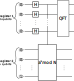
\includegraphics[width=0.65\linewidth]{30_licencjat/tex/figures/shor.png}
    \caption{Quantum circuit of order finding algorithm}
    \label{fig:shor}
\end{figure}
\newpage
We measure the value on the first register, resulting in $x$, in order to find $r$ we need to classically find the best rational approximation for $\frac{x}{m}$, numbers $a$ and $b$ such that $\frac{x}{m}=\frac{a}{b}$. This can be done via the continued fractions algorithm \cite{continued_fractions}. the probability of $x$ being close to $\frac{m}{r}$ is high, but not certain, we must check whether $a^b=1 \mod{n}$, if so we output $b$, otherwise we can rerun the algorithm. 



\subsection{Bringing it together}
In the algorithm we classically check if algorithm is prime, which can be done with AKS algorithm in deterministic, polynomial time \cite{Agrawal2004}. We also compute greatest common divisor which can be solved using Euclid in algorithm $O(\log{(m+n)})$ \cite{cormen2009}.
\\\\
We use the following subroutine recursively until $N$ is prime. In each subsequent call we 
\begin{itemize}
    \item Check if $N$ is not prime, if it is return it.
    \item Check if $N$ is even, if it is return $2$.
    \item Draw number $a$ uniformly from $\{2, \dots, N-1\}$.
    \item Compute the order $s$ of $a$.
    \item Check if $s$ is even and $y^{r/2}\neq \pm1 \mod N$, if not go back to step 3.
    \item Compute $\gcd(a^{s/2}\pm 1,N)$ and return non-trivial factors.
\end{itemize}
We use the check $y^{r/2}\neq \pm1 \mod N$ to ensure that we cannot find two non-trivial factors.\\
